\DiaryEntry{Max-Flow Algorithms, Further Topics I}{2020-06-26}{Algorithms}

\subsection{Other Flow Networks}

In the beginning we defined flow networks as having one source $s$ and one sink $t$ only. In addition, we did not allow for anti-parallel edges between two vertices. Here we show how we can get around these restrictions.

The left Figure below shows a network with several sources and sinks. We can solve this problem by introducing two new vertices, a ``super-source'' $s$, and a ``super-sink''$t$ as shown in the right Figure. The super-source $s$ is connected to the existing sources ($s_1 \ldots s_5$) via edges having infinite capacities; the super-sink is connected to the existing sinks ($t_1 \ldots t_3$) via edges having infinite capacities. We can now solve the maximum-flow problem with any algorithm on this extended flow network.

\begin{figure}[H]
\centering
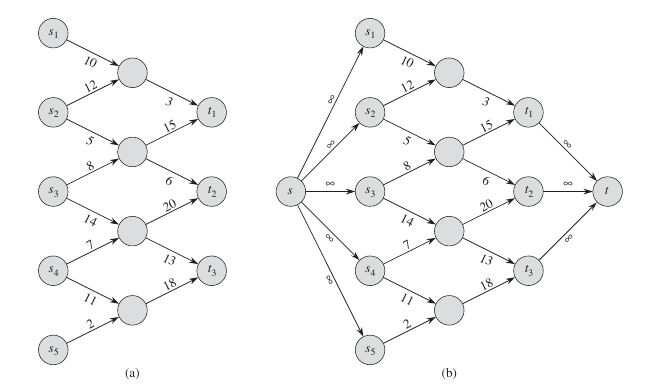
\includegraphics[scale=0.65]{images/max_flow_04_01.png}
\end{figure}

In case of anti-parallel edges, we can introduce an additional vertex which transports one of the flows. The following Figure illustrates the principle. On the left we have two anti-parallel edges between vertices $v_1$ and $v_2$. We extend the flow network by vertex $v'$ as shown on the right: The edge $v_1 \rightarrow v_2$ with capacity $10$ is replaced by the path $v_1 \rightarrow v' \rightarrow v_2$ (each edge having capacity $10$); the edge $v_2 \rightarrow v_1$ with capacity $4$ is not changed. The resulting network is again a flow network and can be solved by max-flow algorithms.

\begin{figure}[H]
\centering
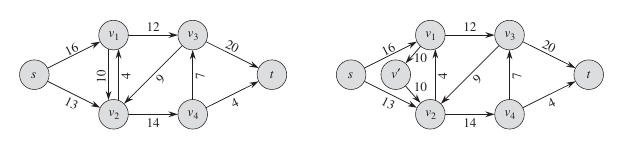
\includegraphics[scale=0.65]{images/max_flow_04_02.png}
\end{figure}


\subsection{Random Graphs}

We ask the question which flow can be transported across a random graph? We consider graphs created by the Erdős–Rényi $G(n,p$) model: The graph is constructed by connecting nodes randomly. Each edge is included in the graph with probability $p$ independent from every other edge.

\paragraph{Fixed Capacity.} In a first step, we assign every edge a capacity of $1$.

The following shows a plot whether a flow between two vertices (vertex $1$ and $100$) exists as a function of $p$. The graph has $100$ vertices and the Figure shows the result over $100$ such random graphs.

It can be seen that for small values of $p$, no flow exists, and at $p \approx 0.02$, there is a threshold above which a flow exists.

\begin{figure}[H]
\centering
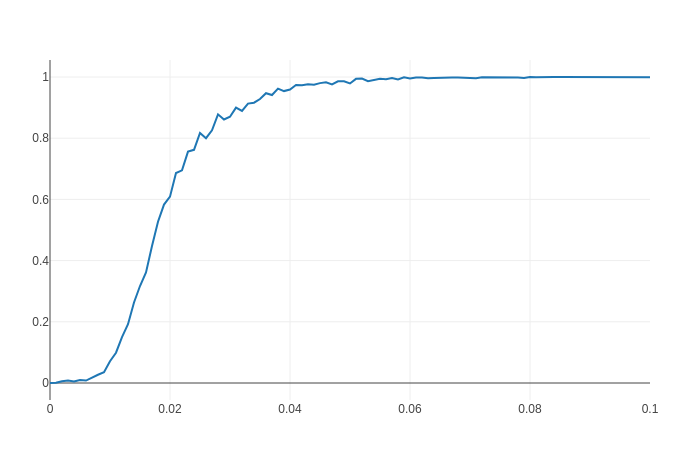
\includegraphics[scale=0.45]{images/max_flow_04_03.png}
\end{figure}

The following Figure shows the mean flow if it exists for a random graph with $100$ vertices as function of $p$. The flow has been averaged over $50$ runs. For $p=1.0$, the graph is fully connected  (with probability $1$). There are $99$ independent paths between any 2 vertices, each of them carrying a flow of $1$, therefore the total flow is $99$. \todo{we need a proof for this}

\begin{figure}[H]
\centering
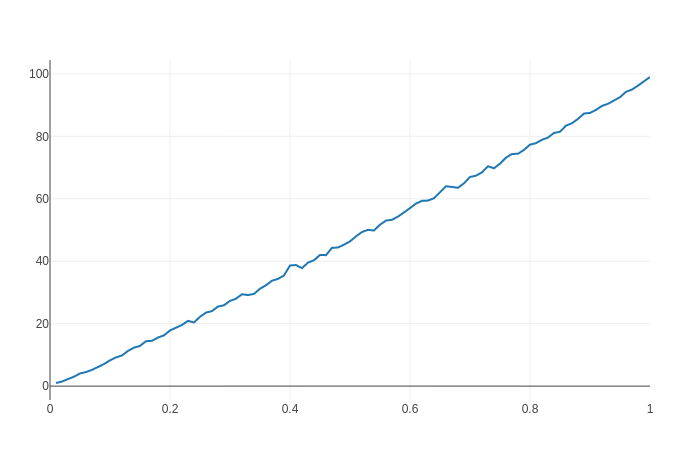
\includegraphics[scale=0.45]{images/max_flow_04_04.png}
\end{figure}

We next show the flow distribution for $p=0.1$ and $p=0.5$.

\begin{figure}[H]
\centering
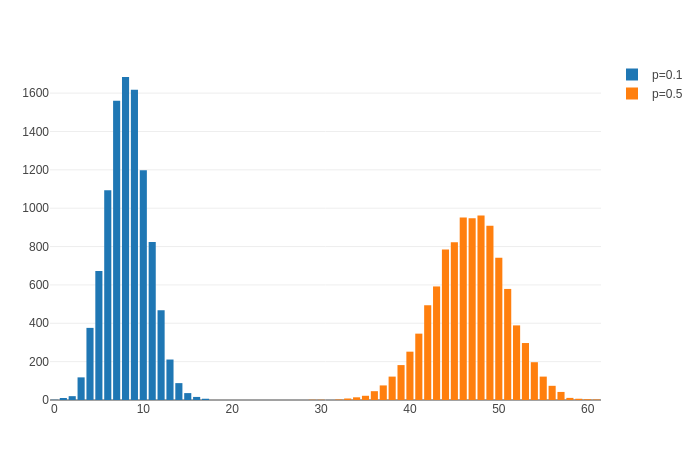
\includegraphics[scale=0.55]{images/max_flow_04_05.png}
\end{figure}

\paragraph{Random Capacity.} We next assign a random capacity to each edge; we chose a uniform distribution on the interval $[0,1]$. 

The following shows a plot whether a flow between two vertices (vertex $1$ and $100$) exists as a function of $p$. It is very similar to the plot with constant capacities.

\begin{figure}[H]
\centering
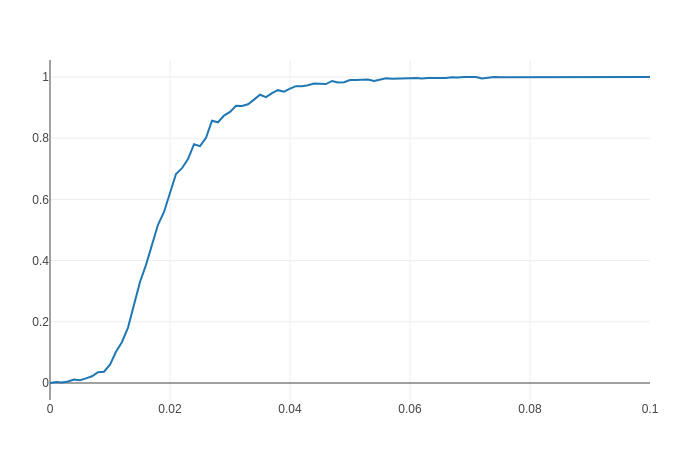
\includegraphics[scale=0.45]{images/max_flow_04_06.png}
\end{figure}

The following Figure shows the mean flow if it exists. Compared to the case with fixed capacities from before, the mean is approximately $50\%$ lower. Intuitively, this makes sense as the mean capacity of each edge is $0.5$; i.e. half the fixed capacity of $1$.

\begin{figure}[H]
\centering
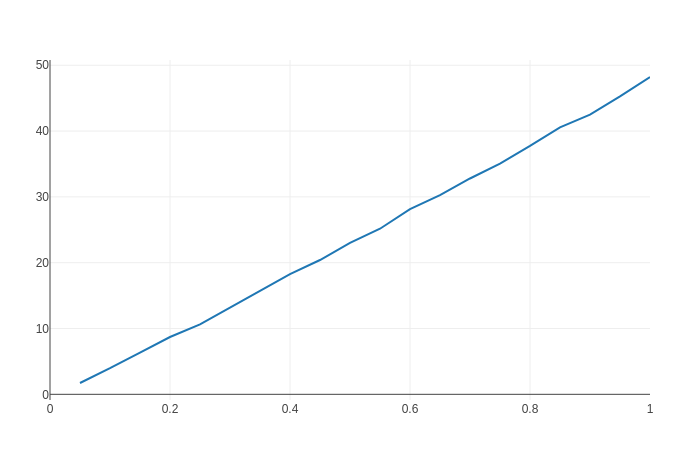
\includegraphics[scale=0.45]{images/max_flow_04_07.png}
\end{figure}

Finally, we plot the flow distribution for $p=0.1$ and $p=0.5$. As seen in the previous plot, the mean is half compared to the case with fixed capacity to $1$. The distribution of the flow looks the same.

\begin{figure}[H]
\centering
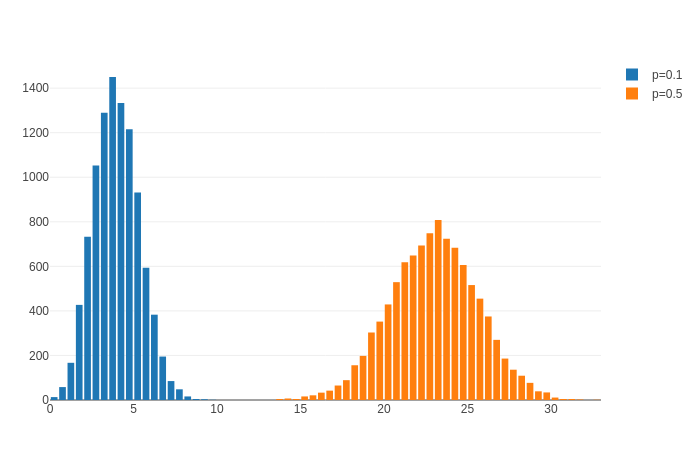
\includegraphics[scale=0.55]{images/max_flow_04_08.png}
\end{figure}


\subsection{Performance}

I used two implementations: (i) the LightsGraphs and LightGraphsFLows packages for Julia and (ii) the NetworkX library for Python. We consider graphs created by an Erdős–Rényi $G(n,p$) model and measure the time to create the graph and run a max-flow algorithm. The following table summarizes the results for different values of $n, p$ of the Julia and Python implementation. The code for the two implementations is given \href{https://github.com/ClemensFMN/JuliaStuff/blob/master/Graphs/rand_graph_perf.jl}{[here} and \href{https://github.com/ClemensFMN/PythonStuff/blob/master/graphs/max_flow_rand_graph.py}{here}.

\vspace{2mm}

\begin{tabular}{|c|c|c|} \hline
  Parameters & Python & Julia \\ \hline
  n = 100, p=0.1 & 25ms & 0.85ms \\
  n = 100, p=0.5 & 115ms & 3.8ms \\
  n = 100, p=0.9 & 184ms & 4.3ms \\
  n = 500, p=0.1 & 633ms & 24ms \\
  n = 500, p=0.5 & 2947ms &129 ms \\ \hline
\end{tabular}

\vspace{2mm}

It can be seen that Julia is considerably faster (by more than one order of magnitude). As a general observation, the algorithms take longer with increasing number of vertices (that's clear) and also with increasing $p$. This is due to the fact that higher values of $p$ create graphs with more edges and the max-flow algorithm needs to consider more augmenting paths.


%%% Local Variables:
%%% mode: latex
%%% TeX-master: "journal"
%%% End:
